\section{Grundbegriffe}
\subsection{Cloud}
Eine Cloud beschreibt das Outsourcen von Rechenaufgaben und Speicher an einem Computer der nicht der lokale Computer ist. Die Cloud kann unterschiedliche Aufgaben übernehmen, meistens sind es Compute und Storage.
\subsection{Compute}
Compute in Cloud Kontext bedeutet das eine Cloud Rechenleistung bereitstellt. Dies kann vielseitig geschehen von einfachen VMs, über Managed Services zum Hosten eigener Anwendungen bis zu SaaS Produkten wie Microsoft 365.
\begin{figure}[H]
    \centering
    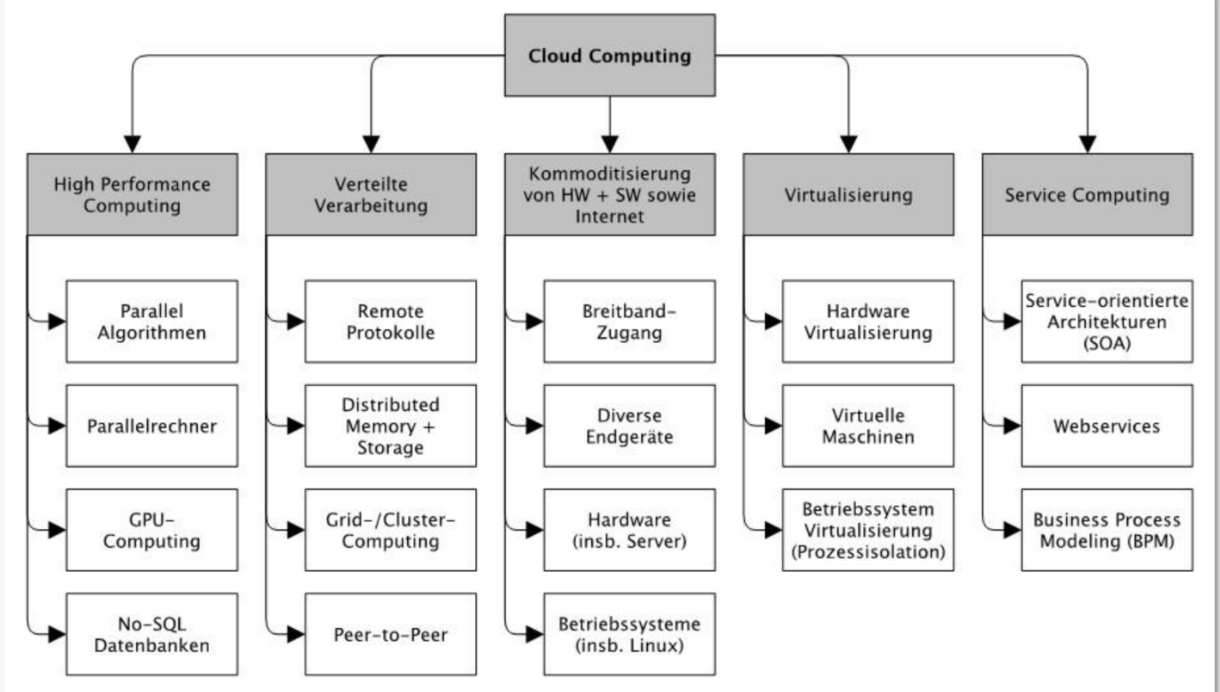
\includegraphics[width=\textwidth]{assets/images/CloudComputingErklaert}
    \caption{Cloud Computing erklärt}
\end{figure}
\subsection{Storage}
Storage in Cloud Kontext bedeutet die Bereitstellung von Speicher. Dies kann geschehen über die verschiedensten Wege zu einem einfachen Cloud Speicher ähnlich zu einer Festplatte, Speicher für Webseiten um Nutzerdaten zu speichern aber auch Speicher integriert in SaaS Produkten wie Microsoft 365 aber auch beispielsweise Netflix.
\subsection{Region}
Eine Cloud-Region ist ein geografischer Bereich, der aus mehreren
Verfügbarkeitszonen besteht. Regionen sind meist nach Himmelsrichtung
oder Lage benannt, zum Beispiel \textit{Deutschland West Central} oder
\textit{North Europe} bei Azure. Die Wahl der Region bestimmt, wo Daten
physisch gespeichert werden (Datenresidenz) und beeinflusst die Latenz
zu den Endnutzern. Jede Region ist physisch und logisch von anderen
Regionen isoliert, sodass ein Ausfall einer Region andere nicht
beeinträchtigt.
\subsection{Verfügbarkeitszonen}
Eine Verfügbarkeitszone (engl. \textit{Availability Zone}) ist eine
physisch getrennte Einheit innerhalb einer Region. Sie besteht aus einem
oder mehreren Rechenzentren mit eigener Stromversorgung, Kühlung und
Netzwerkanbindung. Verfügbarkeitszonen innerhalb einer Region sind über
redundante Hochgeschwindigkeitsverbindungen mit geringer Latenz
verbunden. Durch die Verteilung von Diensten auf mehrere Zonen können
Anwendungen auch bei einem Zonenausfall verfügbar bleiben
(Hochverfügbarkeit).
\subsection{CapEx – Capital Expenditure}
CapEx oder auch Kapitalausgaben sind eine einmalige Investition. Im Cloud Kontext sind das oft der Kauf von Servern. Ein CapEx Ausgabe ist über mehrere Jahre abschreibbar. Das Problem bei einem einmaligen Serverkauf sind die hohen Kosten und das ein Server eine begrenzte Zeit hat in welcher er performant ist. Man kann ab einem gewissen Zeitpunkt nur noch schwierig Hardware nachrüsten.
\subsection{OpEx – Operational Expenditure}
OpEx sind laufende Kosten so wie Cloud Abonnements. OpEx wird direkt verbucht.
\subsection{Skalierung – Scalability}
Skalierung im Cloud Kontext bedeutet Rechenleistung, Speicher und Netzwerkbandbreite dynamisch an sich ändernde Workloads anzupassen. Es wird in zwei Arten unterteilt.
\subsubsection{Horizontale Skalierung}
Bei horizontaler Skalierung wird ein Workload auf mehreren Servern ausgeführt bzw ausgeweitet.
\subsubsection{Vertikale Skalierung}
Ein bestehender Server wird aufgerüstet durch beispielsweise mehr RAM.
\subsection{Hochverfügbarkeit – Availability}
Hochverfügbarkeit bedeutet das eine in der Cloud gehostete Anwendung immer erreichbar ist. Wie viele Ausfälle im Jahr prozentual passieren dürfen ist in einem SLA (Service Level Agreement) festgehalten.
\subsubsection{SLA – Service Level Agreement}
In einem SLA ist Uptime, meist als Nines also z.B. 5 Nines --> 99,999, Reaktion und Lösungszeit, Leistungsparameter, Ausstiegsstrategien und Datenportabilität sowie Sicherheit und Compliance geregelt.
\subsection{Elastizität – Elasticity}
Elastizität im Cloud Kontext bedeutet das eine Anwendung automatisch skaliert werden kann.
